\section{SAES}

\begin{frame}{SAES}
Nibble oriented with block and key size of 16 bits.
\[
    \underbrace{b_0b_1b_2b_3}_\text{$S_0$}  
    \underbrace{b_4b_5b_6b_7}_\text{$S_1$}
    \underbrace{b_8b_9b_{10}b_{11}}_\text{$S_2$}
    \underbrace{b_{12}b_{13}b_{14}b_{15 }}_\text{$S_3$} = 
    \begin{bmatrix}
    S_0 & S_2\\
    S_1 & S_3
    \end{bmatrix} 
    = State
\]
\end{frame}
\begin{frame}{SAES Encryption}
    \begin{figure}[h!]
    \centering
    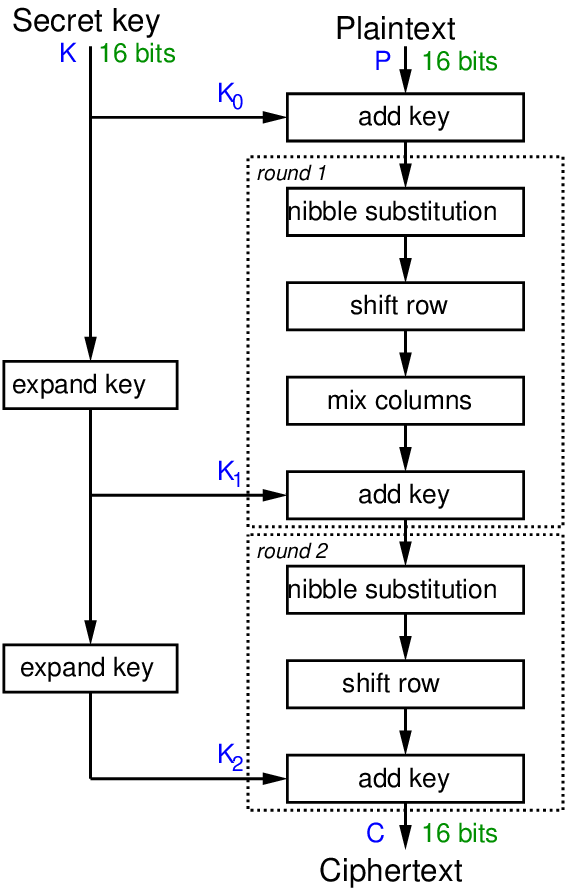
\includegraphics[width=0.4\linewidth]{saes/saes-encryption.png}
    \caption{SAES encryption \footfullcite{Gordon}}
    \label{fig:saes-encryption}
\end{figure}
\end{frame}
\begin{frame}{Sub Nibbles, Shift Rows and Mix Column}
\begin{enumerate}
    \item Compute the multiplicative inverse $x$ i.e. $y = x^{-1}$ in $GF(2^4)$.
    \pause
    \item The result of the sbox is computed using the follows operation:
    
    \begin{equation}\label{eq:sn}
        \begin{bmatrix}
        z_0\\
        z_1\\ 
        z_2\\
        z_3
        \end{bmatrix} = 
        \begin{bmatrix}
        1 & 0 & 1 & 1\\
        1 & 1 & 0 & 1 \\
        1 & 1 & 1 & 0 \\
        0 & 1 & 1 & 1
        \end{bmatrix} 
        \begin{bmatrix}
        y_0 \\ y_1\\
        y_2 \\ y_3
        \end{bmatrix} 
        \oplus
        \begin{bmatrix}
        1  \\ 0\\
        0 \\ 1
        \end{bmatrix} 
    \end{equation}
    \pause
    \item The Shift Rows operation is the same as AES.
    \[
    \begin{bmatrix}
    S_0 & S_2\\
    S_1 & S_3
    \end{bmatrix} \longrightarrow
    \begin{bmatrix}
    S_0 & S_2\\
    S_3 & S_1
    \end{bmatrix} 
\]
\pause
\item SAES mix column.
\[
    \begin{bmatrix}
    S_0'\\
    S_1'\\ 
    \end{bmatrix} = 
    \begin{bmatrix}
    1 & 4 \\
    4 & 1 
    \end{bmatrix}
    \begin{bmatrix}
    S_0\\
    S_1\\ 
    \end{bmatrix}
\]
\item The elements of the matrix are in $\mathbb{F}_{2^4}[x]/(x^2 + 1)$.
\end{enumerate}    
\end{frame}
\begin{frame}{Key Expansion}
    \begin{itemize}
        \item The master key (16 bit) can be thought as 2 bytes $B_0B_1$.
        \pause
        \item 3 Round keys.
        \pause
        \item First round key (16 bit) can be thought as 2 bytes $B_2B_3$.
        \pause
        \item Second round key (16 bit) can be thought as 2 bytes $B_4B_5$.
    \end{itemize}
        \pause
        \begin{codebox}
        \Procname{$\proc{Key Expansion for SAES}(K)$}\label{proc:ke}
        \li $\id{keys} \gets [B_0,B_1,B_2,B_3,B_4,B_5]$
        \li $keys[0] = K[0 \dots 8]$
        \li $keys[1] = K[8 \dots 16]$
        \li  \For $i \gets 2$ \To $5$
        \li     \Do
                        \If $i\%2 == 0$
        \li                 \Then
                                $keys[i] = keys[i-2] \oplus RCON(i/2) \oplus$
        \li                     $keys[i] = keys[i] \oplus Sbox(RotNib(keys[i-1]))$
        \li                \Else
        \li                    $keys[i] = keys[i-2]\oplus keys[i-1]$
                            \End
                \End
        \li \Return $B_0B_1, B_2B_3, B_4B_5$
        \end{codebox}
        \pause
     \begin{itemize}
         \item Round Constant is defined as \[RCON(i) = (x^{i+2} || 0000)\]
     \end{itemize}

\end{frame}
